\section{Syfte och mål}

Syftet med projektet är att konstruera ett system som kör bilar runt en
bana (Se figur~\ref{fig:track_modell}). Till bilbanan finns det 9 ``givare'' som när de passeras skickar en
signal. Med hjälp av tidsskillnaden mellan signalerna kan man räkna ut hur lång
tid det tog för en bil att åka mellan två givare. Bilbanan är även kopplad till
en dator där det finns möjlighet att justera bilarnas gaspådrag med en
spänningstillförsel. Med hjälp av denna information ska ett system skapas som
kör en eller två bilar runt bilbanan på en inställbar varvtid mellan 12 och 15
sekunder, samt gör att bilarna åker i mål så nära varandra i tiden som möjligt.

\begin{figure}
  \centering
  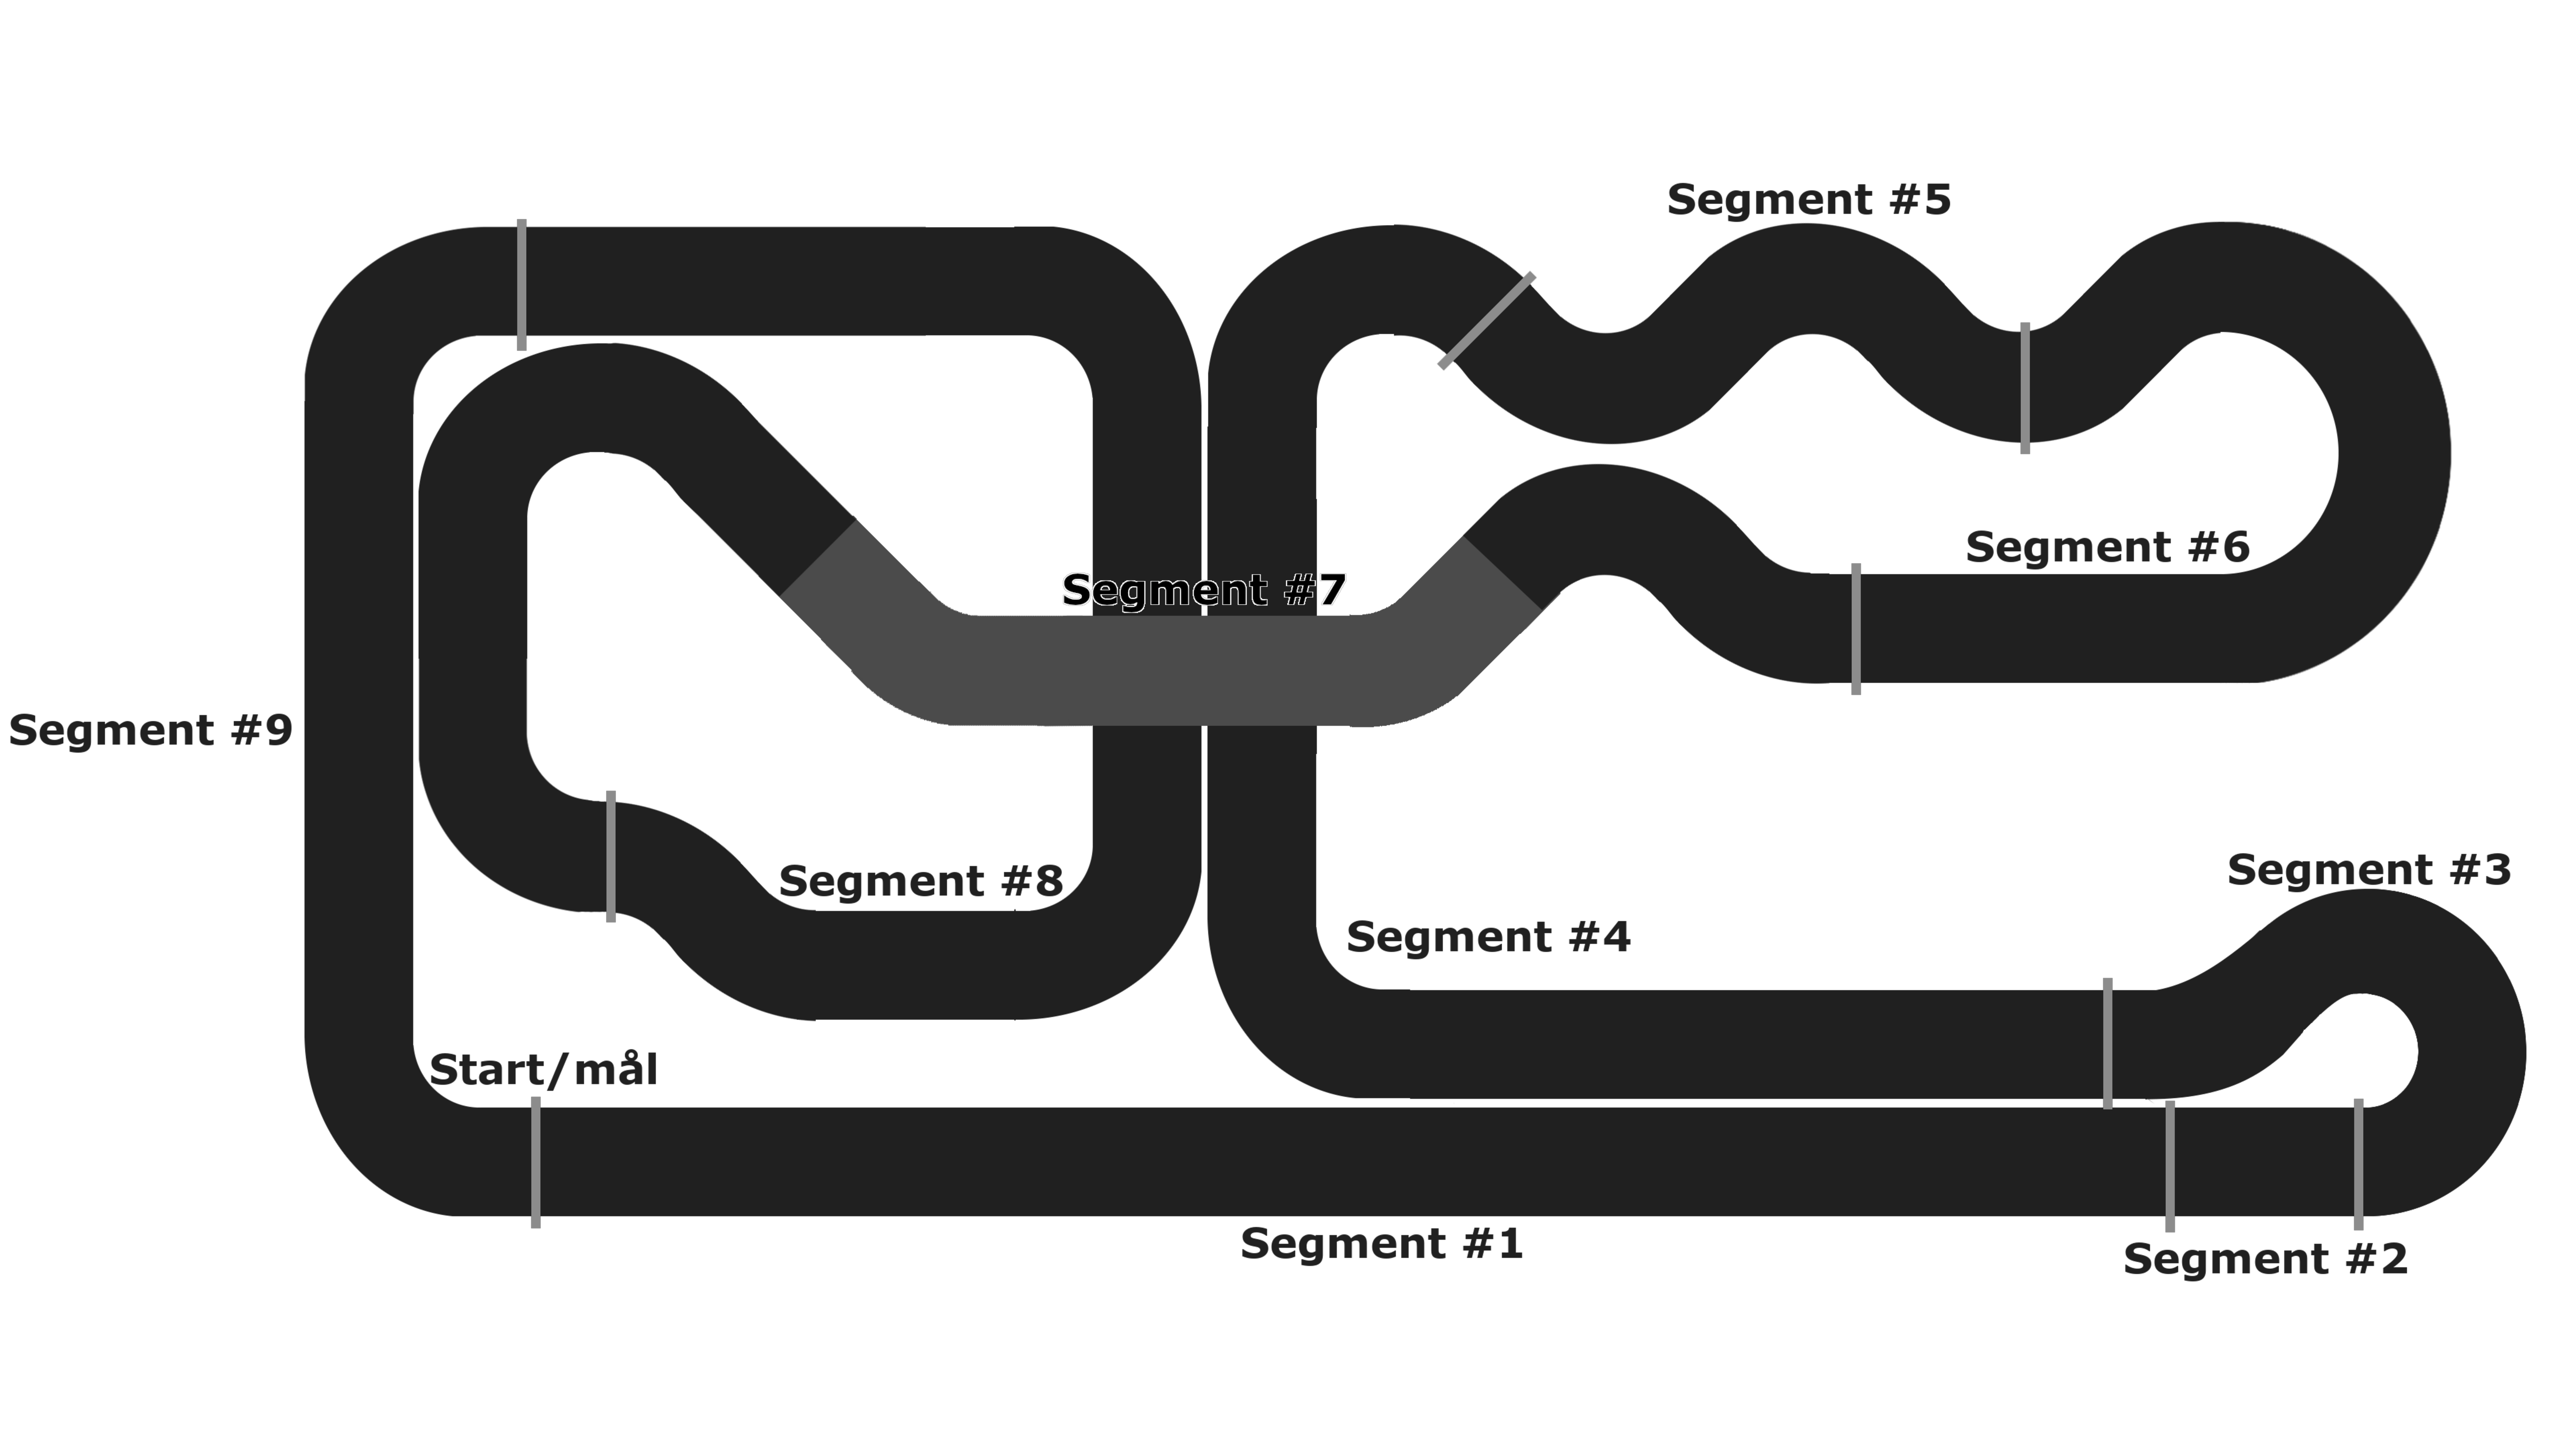
\includegraphics[width=\linewidth]{figures/BanaModell.pdf}
  \caption{En modell av bilbanan.}%
  \label{fig:track_modell}
\end{figure}
